%%%%%%%%%%%%%%%%%%%%%%%%%%%%%%%%%%%%%%%%%%%%%%%%%%%%%%%%%%%%%%%%%%%%%%%%%%%%%%%%
\documentclass[11pt]{article} % Dokumentenklasse

\usepackage[utf8]{inputenc} % Textkodierung: UTF-8
\usepackage[T1]{fontenc} % Zeichensatzkodierung

\usepackage[USenglish]{babel}% http://ctan.org/pkg/babel
\usepackage{graphicx} % Grafiken
\usepackage[absolute]{textpos} % Positionierung

% Schriftart Helvetica:
\usepackage[scaled]{helvet}
\renewcommand{\familydefault}{\sfdefault}

\usepackage{calc} % Berechnungen
\usepackage{tabto} % Tabulatoren
\usepackage{parskip}

\usepackage{enumitem}

% Debugging:
%\usepackage{layout} % Layout-Informationen
%\usepackage{printlen} % Längenwerte ausgeben

%%%%%%%%%%%%%%%%%%%%%%%%%%%%%%%%%%%%%%%%%%%%%%%%%%%%%%%%%%%%%%%%%%%%%%%%%%%%%%%%
% EINSTELLUNGEN
%%%%%%%%%%%%%%%%%%%%%%%%%%%%%%%%%%%%%%%%%%%%%%%%%%%%%%%%%%%%%%%%%%%%%%%%%%%%%%%%

% Seitenränder:
\newcommand{\SeitenrandOben}{43.5mm}
\newcommand{\SeitenrandRechts}{20mm}
\newcommand{\SeitenrandLinks}{20mm}
\newcommand{\SeitenrandUnten}{10mm}

\newcommand{\UniversitaetLogoBreite}{19mm}
\newcommand{\UniversitaetLogoHoehe}{1cm}

\usepackage[a4paper,
top=\SeitenrandOben,
bottom=\SeitenrandUnten,
inner=\SeitenrandLinks,
outer=\SeitenrandRechts,
foot=0cm,
head=0cm
]{geometry}

\textblockorigin{\SeitenrandLinks}{\SeitenrandOben} % Ursprung für Positionierung

\setlength{\parindent}{0pt}
%\setlength{\baselineskip}{32pt}
\setlength{\parskip}{\baselineskip}
\TabPositions{4cm}
\pagestyle{empty}

%%%%%%%%%%%%%%%%%%%%%%%%%%%%%%%%%%%%%%%%%%%%%%%%%%%%%%%%%%%%%%%%%%%%%%%%%%%%%%%%
% General stuff
%%%%%%%%%%%%%%%%%%%%%%%%%%%%%%%%%%%%%%%%%%%%%%%%%%%%%%%%%%%%%%%%%%%%%%%%%%%%%%%%
\newcommand{\Problem}[1]{\paragraph*{Problem #1:}\qquad}
\newcommand{\Topic}[1]{
	\newpage
	\section*{#1}}

\newcommand{\Given}{\textbf{Given:\qquad\qquad}}
\newcommand{\Searched}{\textbf{Searched:\qquad}}
\newcommand{\Solution}{\textbf{Solution:\qquad}}

%%%%%%%%%%%%%%%%%%%%%%%%%%%%%%%%%%%%%%%%%%%%%%%%%%%%%%%%%%%%%%%%%%%%%%%%%%%%%%%%
% Math stuff
%%%%%%%%%%%%%%%%%%%%%%%%%%%%%%%%%%%%%%%%%%%%%%%%%%%%%%%%%%%%%%%%%%%%%%%%%%%%%%%%
\usepackage{amsmath}
\usepackage{amssymb}

\newcommand{\R}{\mathbb{R}}
\newcommand{\Vector}[1]{\R^{#1}}
\newcommand{\Matrix}[2]{\R^{#1 \times #2}} % !!! DON'T TOUCH !!!
%%%%%%%%%%%%%%%%%%%%%%%%%%%%%%%%%%%%%%%%%%%%%%%%%%%%%%%%%%%%%%%%%%%%%%%%%%%%%%%%


\newcommand{\ExerciseNumber}{03}

\newcommand{\PersonOne}{Marcel Bruckner (03674122)}
\newcommand{\PersonTwo}{Julian Hohenadel (03673879)}
\newcommand{\PersonThree}{Kevin Bein (03707775)}

%%%%%%%%%%%%%%%%%%%%%%%%%%%%%%%%%%%%%%%%%%%%%%%%%%%%%%%%%%%%%%%%%%%%%%%%%%%%%%%%
% DOKUMENT
%%%%%%%%%%%%%%%%%%%%%%%%%%%%%%%%%%%%%%%%%%%%%%%%%%%%%%%%%%%%%%%%%%%%%%%%%%%%%%%%

\begin{document}

%%%%%%%%%%%%%%%%%%%%%%%%%%%%%%%%%%%%%%%%%%%%%%%%%%%%%%%%%%%%%%%%%%%%%%%%%%%%%%%%
\begin{textblock*}{\UniversitaetLogoBreite}[1,0](\textwidth-1mm, 2cm-\SeitenrandOben)%
	\raggedleft
\includegraphics{../Ressources/Universitaet_Logo_RGB.pdf}%
\end{textblock*}


\begin{textblock*}{\textwidth}[0,0](0cm, 0cm)%
	{\fontsize{24pt}{26pt}\selectfont\textbf{Exercise}}
	
	\vspace*{14pt}
	{\fontsize{18pt}{27pt}\selectfont\textbf{\ExerciseNumber}}
\end{textblock*}

\vspace*{92.2mm}
\fontsize{15pt}{17.5pt}\selectfont%
TUM Department of Informatics

\renewcommand{\baselinestretch}{1.47}
\normalsize\selectfont
\vspace*{17.1mm}
\textbf{Supervised by}\tab
\begin{minipage}[t]{\textwidth-\CurrentLineWidth}
	Prof. Dr. Stephan Günnemann\\
	Informatics 3 - Professorship of Data Mining and Analytics\strut
\end{minipage}

\vspace*{4.3mm}
\textbf{Submitted by}\tab
\begin{minipage}[t]{\textwidth-\CurrentLineWidth}
	\PersonOne\\
	\PersonTwo\\
	\PersonThree
\end{minipage}

\vspace*{-1mm}
\textbf{Submission date}\tab 
\begin{minipage}[t]{\textwidth-\CurrentLineWidth}
	Munich, \today
\end{minipage}
\newpage % !!! DON'T TOUCH !!!
%%%%%%%%%%%%%%%%%%%%%%%%%%%%%%%%%%%%%%%%%%%%%%%%%%%%%%%%%%%%%%%%%%%%%%%%%%%%%%%%

%%%%%%%%%%%%%%%%%%%%%%%%%%%%%%%%%%%%%%%%%%%%%%%%%%%%%%%%%%%%%%%%%%%%%%%%%%%%%%%%
% !!! HOMEWORK STARTS HERE !!!
%%%%%%%%%%%%%%%%%%%%%%%%%%%%%%%%%%%%%%%%%%%%%%%%%%%%%%%%%%%%%%%%%%%%%%%%%%%%%%%%
%
\Topic{Optimizing Likelihoods: Monotonic Transforms}
%
\Problem{1}
\[ f_1(\theta) = \theta^t(1-\theta)^h \]
\[ f_2(\theta) = \log(\theta^t(1-\theta)^h) \]
\begin{align*}
\pd{\theta} f_1(\theta) &= t \theta^{t-1}(1-\theta)^h + \theta^t \pd{\theta}\left((1-\theta)^h\right) \\
&= t\theta^{t-1}(1-\theta)^h - \theta^t  h (1-\theta)^{h-1}
& \\
\pds{\theta} f_1(\theta) &= t \cdot \pd{\theta}\left(\theta^{t-1}(1-\theta)^h \right) - h \cdot \pd{\theta}\left(\theta^t (1-\theta)^{h-1}\right) \\
&= t \cdot \left((t-1)\theta^{t-2}(1-\theta)^h - \theta^{t-1}h(1-\theta)^{h-1}\right) \\
&+ h \cdot \left(t\theta^{t-1} (1-\theta)^{h-1} - \theta^t (h-1)(1-\theta)^{h-2}\right) \\
& \\
\pd{\theta} f_2(\theta) &= \pd{\theta}\left(\log(\theta^t) + \log((1-\theta)^h)\right) \\
&= \pd{\theta}\left(\log(\theta^t) \right) + \pd{\theta}\left(\log((1-\theta)^h)\right) \\
&= t \cdot \pd{\theta}\left(\theta\right) + h \cdot \pd{\theta}\left(\log(1-\theta)\right) \\
&= \frac{t}{\theta} - \frac{h}{1-\theta} \\
& \\
\pds{\theta} f_2(\theta) &= \pd{\theta}\left(\frac{t}{\theta}\right) - \pd{\theta}\left(\frac{h}{1-\theta}\right) \\
&= \frac{0\cdot \theta - t\cdot 1}{\theta^2} - \frac{0\cdot (1-\theta) - h \cdot (-1)}{(1-\theta)^2} \\
&= -\frac{t}{\theta^2} - \frac{h}{(1-\theta)^2}
\end{align*}
%
%
\newpage
%
\Problem{2}
%
\begin{quote}
"Monotonic functions preserver critical points"
\end{quote}
\begin{flushleft}
Since $\log$ is a monotonic transformation, the function will yield the same values when plugged into $\underset{\theta}{\arg\max}$:
\[ \argmax_\theta f(\theta) = \argmax_\theta \log f(\theta) \]
%\begin{align*}
%&f(x_1, \ldots, x_n | \theta) = f(x_1 | \theta) \cdot \ldots \cdot f(x_n | \theta) \\
%\Rightarrow & \log(f(x_1, \ldots, x_n | \theta)) = \log(f(x_1)) \cdot \ldots \cdot \log(f(x_n)) = \log(f(x|\theta)) \\
%\Rightarrow & \pd{\theta} \left( \log(f(x|\theta))\right) = \frac{\pd{\theta}{f(x)}}{f(x)}
%\end{align*}
Considering problem 1 and the fact that log converts exponents to factors (which also increases the numerical stabillity), computing the log-likelihood is faster and yields more compact functions which can then be maximized.
\end{flushleft}
%
%
\Topic{Properties of MLE and MAP}
%
%
\Problem{3}
%
\begin{align*}
  Beta(6,4) &= \left(\frac{\Gamma(6+4)}{\Gamma(6)\Gamma(4)} \cdot \theta^{6-1} \cdot (1-\theta)^{4-1}\right) \\
  &= \frac{9!}{5! \cdot 4!} \cdot \theta^5\cdot  (1-\theta)^3 \\
  &= 126 \cdot \theta^5 \cdot (1-\theta)^3
\end{align*}
\begin{align*}
  \theta_{\text{MAP}} &= \argmax_\theta p(\theta|f) \\
  &= \argmax_\theta \frac{p(f|\theta) \cdot p(\theta)}{p(f)} \\
  &= \argmax_\theta p(f|\theta) \cdot p(\theta) \\
  &= \argmax_\theta \left(\theta^{\mathbb{I}[f=T]} \cdot (1-\theta)^{\mathbb{I}[f=H]}\right) \cdot \left(126 \cdot \theta^5 \cdot (1-\theta)^3\right) \\
  &= \argmax_\theta \theta^{M+5} \cdot (1-\theta)^{N+3} \\
  &= \argmax_\theta \log\left(\theta^{M+5} \cdot (1-\theta)^{N+3}\right) \\ 
  &= \argmax_\theta (M+5) \log(\theta) + (N+3) \log(1-\theta)
\end{align*}
\begin{align*}
  \Rightarrow \; & \pd{\theta} (M+5) \log(\theta) + (N+3) \log(1-\theta) = \frac{M+5}{\theta} - \frac{N-3}{1-\theta} \overset{!}{=} 0 \\
  \Rightarrow \; & \theta_\text{MAP} = \frac{M+5}{M+N+8}
\end{align*}
\begin{align*}
  \theta_\text{MAP} \overset{!}{=} 0.75 = \frac{3}{4} = \frac{30}{40} \\
  \Rightarrow \; M=25, N=40-25-8= 7
\end{align*}
(In general, the solution is $M=3N+1$)
%
%
\newpage
\Problem{4}
%
\begin{flushleft}
Given are $X \sim Bern$, $P(\theta) \sim Beta$ and $P(D|\theta) \sim Binomial$.
The expecterd mean of the prior (Beta distribution) is $\E[\theta] = \frac{a}{a+b}$. The maximum likelihood estimate is given by $\E[\theta_\text{MLE}] = \frac{m}{N} = \frac{m}{m+l}$. We now identify the posterior mean distribution:
\end{flushleft}
\begin{align*}
P(\theta|D) &= \frac{P(D|\theta) P(\theta)}{P(D)} \\
&= \left(\binom{N}{m} \theta^m (1-\theta)^{N-m}\right) \cdot \left(\frac{\Gamma(a+b)}{\Gamma(a)\Gamma(b)} \theta^{a-1} (1-\theta)^{b-1}\right) \\
&= \binom{N}{m} \frac{\Gamma(a+b)}{\Gamma(a)\Gamma(b)} \cdot \theta^{m+a-1} \cdot (1-\theta)^{N-m+b-1} \\
&\propto \theta^{m+a-1} \cdot (1-\theta)^{N-m+b-1} \\
&\propto Beta(\theta | m+a, N-m+b) = Beta(\theta | m+a, l+b)
\end{align*}
Looking up the mean of the Beta distribution yields the mean of the posterior distribution:
\[ \E[\theta|D] = \E[\theta|m,N,a,b] = \frac{m+a}{m+a+N-m+b} = \frac{a+m}{a+b+m+l} \]
Refactoring the mean
\begin{align*}
  \frac{a+m}{a+b+m+l} &= \frac{a}{a+b+m+l} + \frac{m}{a+b+m+l} \\
  &= \underbrace{\frac{a+b}{a+b+m+l}}_{\lambda} \cdot \frac{a}{a+b} + \underbrace{\frac{m+l}{a+b+m+l}}_{(1-\lambda)} \cdot \frac{a}{m+l} \\
  &= \lambda \cdot \frac{a}{a+b} + (1-\lambda)\cdot\frac{m}{m+l} \\
  &= \lambda \cdot \E[\theta] + (1-\lambda) \cdot \E[\theta_\text{MLE}]
\end{align*}
shows that the posterior mean lies between the prior mean and the maximum likelihood estimate for $\theta$.
%
%
\Topic{Programming Task}
%
\Problem{5}
%
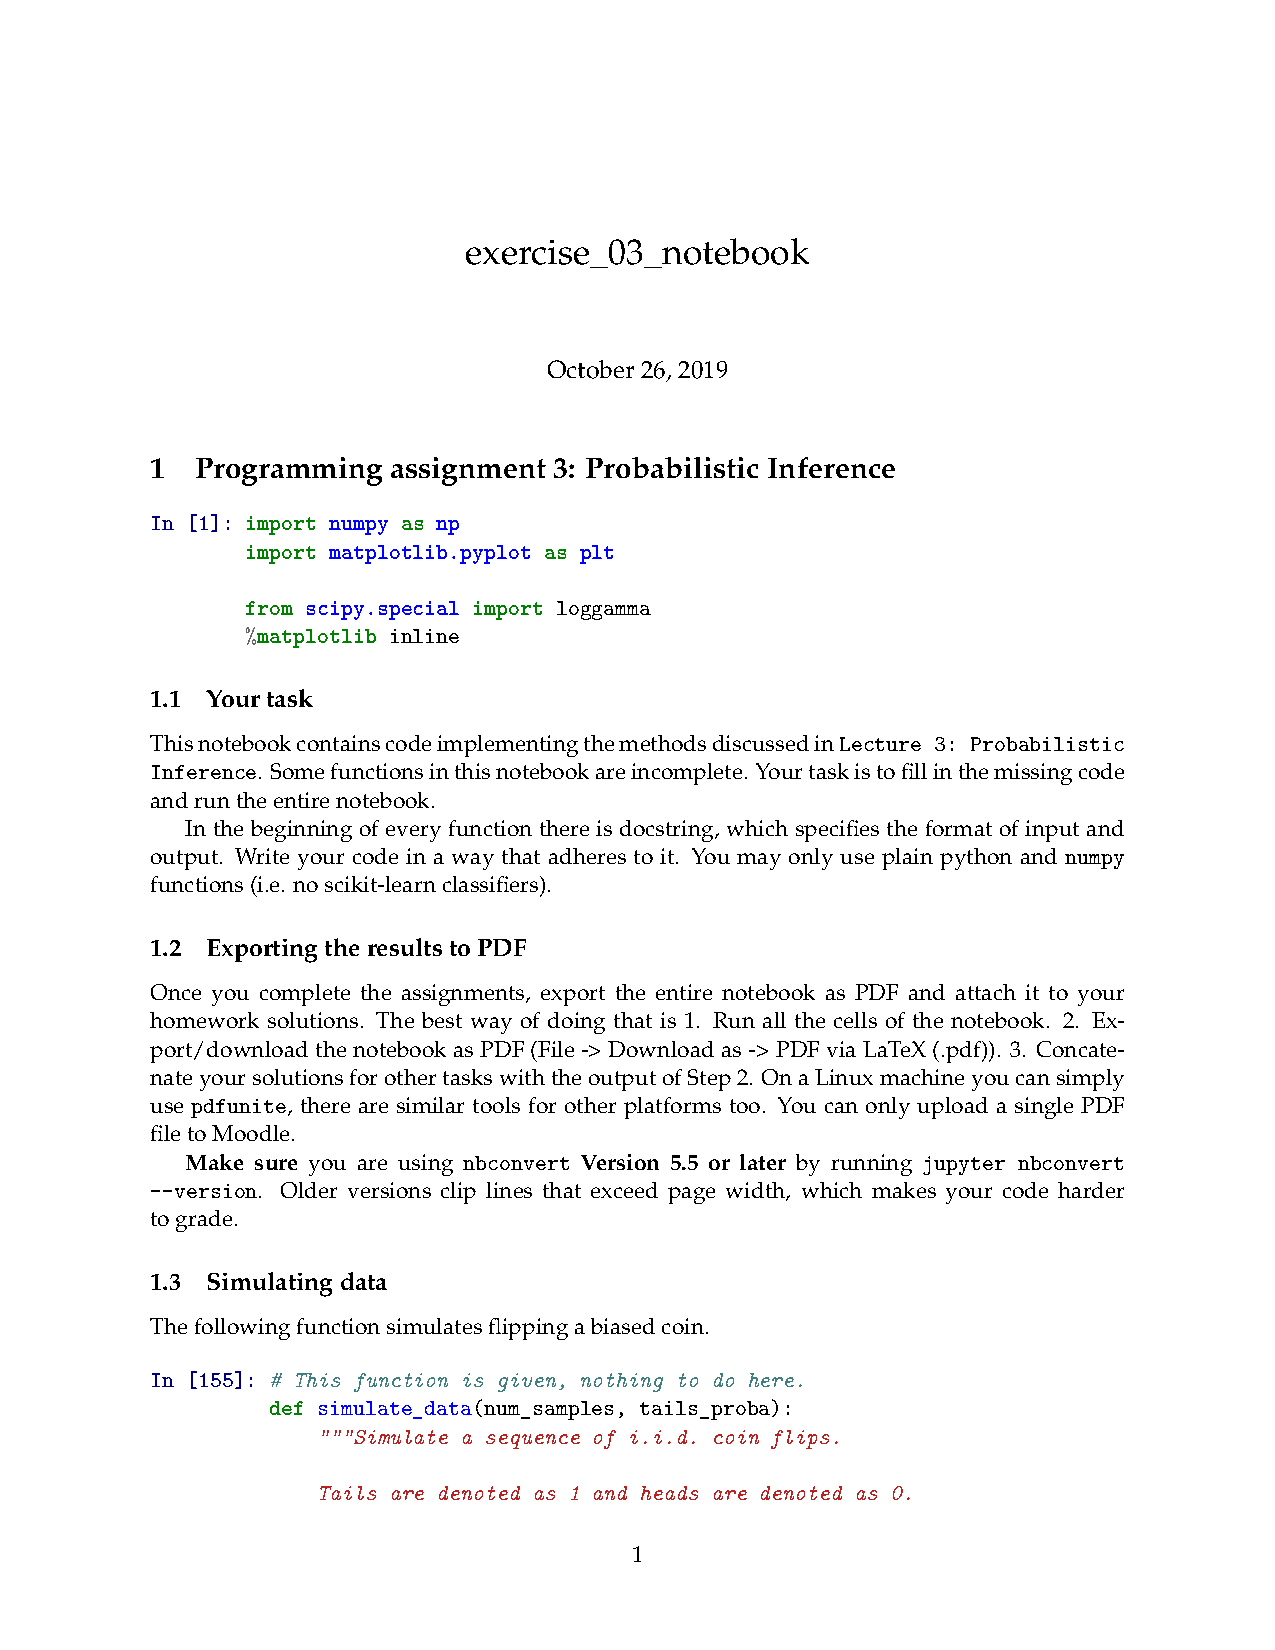
\includepdf[pages=-]{exercise_03_notebook.pdf}
%
%%%%%%%%%%%%%%%%%%%%%%%%%%%%%%%%%%%%%%%%%%%%%%%%%%%%%%%%%%%%%%%%%%%%%%%%%%%%%%%%
% !!! HOMEWORK ENDS HERE !!!
%%%%%%%%%%%%%%%%%%%%%%%%%%%%%%%%%%%%%%%%%%%%%%%%%%%%%%%%%%%%%%%%%%%%%%%%%%%%%%%%

%%%%%%%%%%%%%%%%%%%%%%%%%%%%%%%%%%%%%%%%%%%%%%%%%%%%%%%%%%%%%%%%%%%%%%%%%%%%%%%%
\newpage

\vspace*{-15.8mm}
\fontsize{19pt}{21pt}\selectfont

\vspace{25.3mm}
Appendix

\normalsize\selectfont
\vspace{13.2mm}
We confirm that the submitted solution is original work and was written by us without further assistance. Appropriate credit has been given where reference has been made to the work of others.

\vspace{18.1mm}
\rule[-3.7mm]{\linewidth}{0.5pt}
Munich, \today, Signature \PersonOne

\vspace{18.1mm}
\rule[-3.7mm]{\linewidth}{0.5pt}
Munich, \today, Signature \PersonTwo

\vspace{18.1mm}
\rule[-3.7mm]{\linewidth}{0.5pt}
Munich, \today, Signature \PersonThree
 % !!! DON'T TOUCH !!!
%%%%%%%%%%%%%%%%%%%%%%%%%%%%%%%%%%%%%%%%%%%%%%%%%%%%%%%%%%%%%%%%%%%%%%%%%%%%%%%%

\end{document}
